\chapter{Trigonométrie circulaire}\label{chap_fcttrigo}

\section{Fonctions trigonométriques}
	

	\subsection{Sinus et cosinus}\label{subsec_sincos}
		\begin{defi}[Cercle trigonométrique]
			Soit $(O,I,J)$ un repère orthonormé direct. On définit le cercle trigonométrique $\S$ comme étant le cercle de centre $O$ et de rayon $1$.
		\end{defi}
		\paragraph{Remarques.} 

		\begin{enumerate}
			\item Usuellement, dans les livres de mathématiques, on note $\S_1$ le cercle de rayon 1, $\S_2$ la sphère de rayon 1, $S_3$ l'hypersphère de rayon 1. Les nombres des indices correspondent aux dimensions des objets\,: le cercle $\S_1$ est un objet de dimension 1, la sphère $\S_2$ est un objet de dimension 2, l'hypersphère $\S_3$ est un objet de dimension 3, etc. Comme il ne sera que question de $\S_1$ ici, afin d'alléger les notations, on note par convention $\S=\S_1$.
		
			\item Si l'on se donne plusieurs repères orthonormés du plan, alors on peut envisager plusieurs cercles trigonométriques dans le plan.
		\end{enumerate}

		\begin{defi}[Cosinus et sinus]
			Soit $\S$ le cercle trigonométrique de centre $O$. Soit $(O;I;J)$ un repère orthonormé direct unitaire. On note $\S^+$ le demi-cercle obtenu par l'intersection de $\S$ et du demi-plan fermé d'extrémité $(OI)$ et qui contient $J$. On note $\S^-$ le demi-cercle obtenu par l'intersection de $\S$ et du demi-plan ouvert d'extrémité $(OI)$ qui ne contient pas $J$, à savoir $\S^-=\S-(\S^+-(OI))$ (voir figure \ref{fig_def_trigo_Spm}). 

			Soit $M\in\S^+$. Alors $\widehat{IOM}$ est un angle saillant dont la mesure est la longueur de l'arc $\wideparen{IM}$. Le point $M$ est déterminé par la mesure de l'angle $\widehat{IOM}$. Ses coordonnées sont donc des fonctions de cet angle. 
			Lorsque $M\in\S^-$, $\widecheck{IOM}$ est un angle rentrant dont la mesure est $2\pi$ moins la longueur de l'arc $\wideparen{IM}$. (Voir figure \ref{fig_def_trigo_Spm})

			Dans les conditions énoncées ci-dessus, on aura deux cas possibles\,:
			\begin{enumerate}
			 	\item Si $M\in\S^+$\,:
 				\begin{itemize}[label=\textbullet]
					\item on appelle cosinus de l'angle $\widehat{IOM}$, et on note $\cos\widehat{IOM}$, l'abscisse du point $M$,
					\item on appelle sinus de l'angle $\widehat{IOM}$, et on note $\sin\widehat{IOM}$, l'ordonnée du point $M$.
				\end{itemize}
				\item Si $M\in\S^--(OI)$\,:
				\begin{itemize}[label=\textbullet]
					\item on appelle cosinus de l'angle $\widecheck{IOM}$, et on note $\cos\widecheck{IOM}$, l'abscisse du point $M$,
					\item on appelle sinus de l'angle $\widecheck{IOM}$, et on note $\sin\widecheck{IOM}$, l'ordonnée du point $M$.
				\end{itemize}
			 \end{enumerate} 
			Autrement dit\,: 
			\begin{equation}
				M(x,y)\in\S^+ \Leftrightarrow \(\cos\widehat{IOM}=x \wedge \sin\widehat{IOM}=y\).
			\end{equation}
			\begin{equation}
				M(x,y)\in\S^- \Leftrightarrow \(\cos\widecheck{IOM}=x \wedge \sin\widecheck{IOM}=y\).				
			\end{equation}
		\end{defi}

		\begin{figure}
			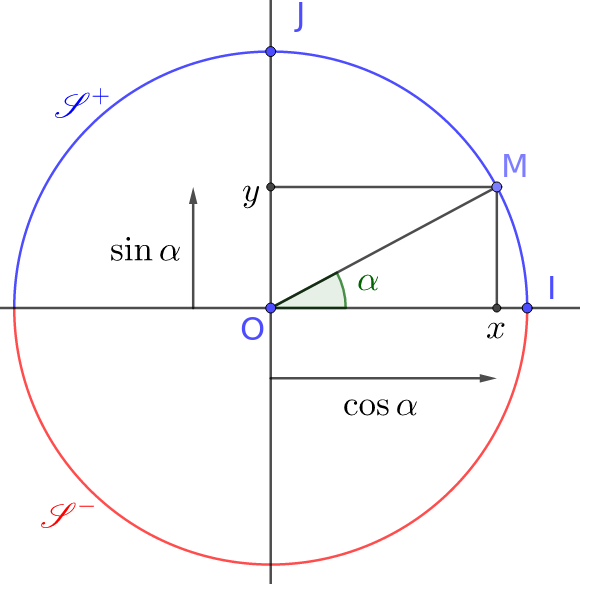
\includegraphics[width=0.46\textwidth]{image/fct_trigo/def_trigo_sp.png}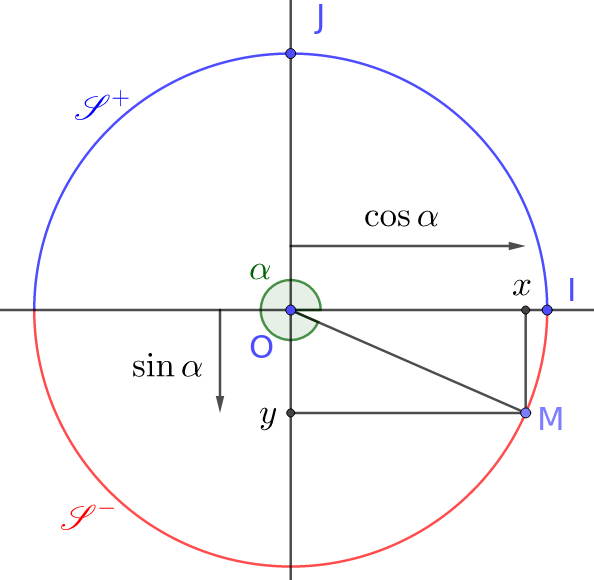
\includegraphics[width=0.46\textwidth]{image/fct_trigo/def_trigo_sm.png}
			\caption{À gauche\,: définition des fonctions trigonométriques dans le cas où $M\in\S^+$. À droite\,: idem, dans le cas où $M\in\S^-$.}
			\label{fig_def_trigo_Spm}
		\end{figure}

		\paragraph{Remarque.} Cette définition est un peu lourde, et on peut avantageusement la simplifier en considérant un angle orienté $\alpha=\ovr{(O,I,M)}$ qui vérifie $-\pi<\alpha\le \pi$. En effet, si l'on part du point $I$ et que l'on effectue une rotation orientée de centre $O$ et d'angle $\alpha$ avec $-\pi<\alpha<0$, le résultat de cette rotation se situera sur $\S^--(OI)$ et on sera dans le point 2 de la définition\,; si $0\le\alpha\le\pi$, on se situe dans $\S^+$ et dans ce cas on est dans le point 1 de la définition. On peut donc avantageusement récrire cette définition\,:

		\begin{defi}[Cosinus et sinus orientés]
			Soit $M\in\S$. Alors il existe un unique nombre réel $\alpha\in]-\pi,\pi]$ tel que $M$ soit l'image de la rotation de centre $O$ et d'angle orienté $\alpha$. $M$ ayant pour coordonnées $(x,y)$, on pose par convention
			\begin{equation}
				\cos\alpha = x,\quad \sin\alpha = y.
			\end{equation}
		\end{defi}

		\begin{figure}
			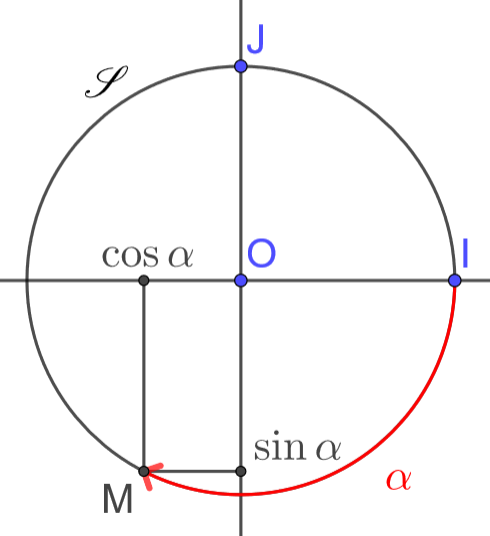
\includegraphics[width=0.37\textwidth]{image/fct_trigo/cossin_oriente_m.png}\hspace{0.1cm}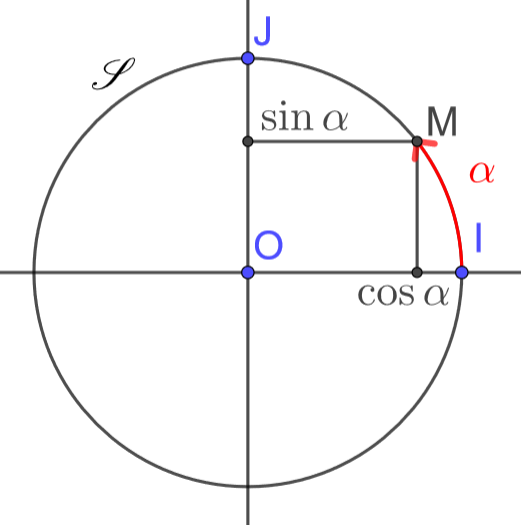
\includegraphics[width=0.4\textwidth]{image/fct_trigo/cossin_oriente_p.png}
			\caption{Illustration de la définition des fonctions trigonométriques dans le cas des angles orientés. À gauche, $-\pi<\alpha<-\frac{\pi}{2}$. Dans ce cas, $\cos\alpha<0$ et $\sin\alpha<0$. À droite, $0<\alpha<\frac{\pi}{2}$. Dans ce cas, $\cos\alpha>0$ et $\sin\alpha>0$.}
		\end{figure}

		\paragraph{Remarque.} On peut en fait définir les fonctions trigonométriques sur tout intervalle de la forme $]x,x+2\pi]$, ou $[x,x+2\pi[$, si l'on souhaite parcourir le cercle trigonométrique une seule fois et avoir une relation univoque entre l'angle et la position du point sur le cercle. Certains livres définissent les fonctions trigonométriques sur $[0,2\pi[$.

		\vspace{0.3cm}

		Il est également possible de définir les fonctions trigonométriques sur $\R$ en ramenant tout nombre réel à un nombre de l'intervalle $]-\pi,\pi]$. En effet, en vertu de la propriété archimédienne de $\R$, pour tout nombre réel $r$, il existe un entier relatif $k$ tel que $(2k-1)\pi<r\le (2k+1)\pi$. Dans ce cas, on dit que le nombre $r$ est congru à $r'=r-2k\pi$ modulo $2\pi$\,; alors $r'\in]-\pi,\pi]$. En fait, dire que $r$ et $r'$ sont congrus modulo $2\pi$ revient à dire que les rotations d'angles $r$ et $r'$ sont identiques à $k$ tours complets près (voir figure \ref{fig_congr}). Formellement, on a la définition suivante\,:
		\begin{defi}[Congruence modulo $2\pi$]
			Soient $u,v\in\R$. $u$ et $v$ sont congrus modulo $2\pi$ signifie qu'il existe un entier relatif $k$ tel que $u=v+2k\pi$. Formellement\,:
			\begin{equation}
				u\equiv v [2\pi] \Leftrightarrow \exists k\in\Z, u=v+2k\pi.
			\end{equation}
		\end{defi}

		\begin{figure}
			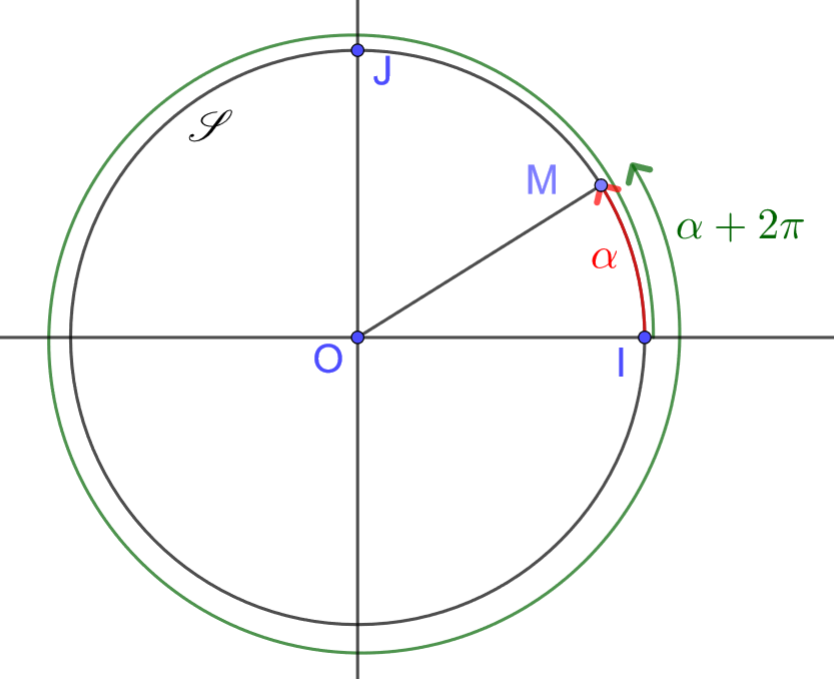
\includegraphics[width=0.5\textwidth]{image/fct_trigo/congr.png}
			\caption{Illustration de la congruence modulo $2\pi$\,: on voit que les $\alpha$ et $\alpha+2\pi$ correspondent au même point sur le cercle trigonométrique, puisque l'angle $2\pi$ correspond à un tour complet.}
			\label{fig_congr}
		\end{figure}

		\paragraph{Remarque.} L'extension de la congruence modulo n'importe quel nombre est triviale.


		Ainsi, en se ramenant à des valeurs comprises entre $-\pi$ et $\pi$, on peut prolonger les fonctions cosinus et sinus au delà de leur intervalle de définition initial. Cela nous donne donc la définition suivante\,:

		\begin{defi}[Cosinus et sinus sur $\R$]
			Soit $u$ un nombre réel. Alors il existe un unique nombre réel $v$ tel que $(u\equiv v\mod[2\pi])\wedge(-\pi<v\le\pi)$, et dans ce cas, on pose
			\begin{equation}
				\cos u= \cos v,\quad \sin u=\sin v.
			\end{equation}
		\end{defi}

		\paragraph{Explication visuelle.} Si l'on souhaite calculer le cosinus et le sinus d'un angle $u$, où $u\notin]-\pi,\pi]$, géométriquement, ramener $u$ à un angle compris entre $-\pi$ et $\pi$ revient à \guil{enrouler} un segment de longueur $u$ autour du cercle trigonométrique et regarder où se situe l'extrémité du segment\footnote{C'est cette idée que nous avons représentée dans la figure \ref{fig_congr}, mais une animation geogebra montre explicitement cet \guil{enroulement}\,: \url{https://www.geogebra.org/m/Ry4j9ZT2}}. 

	\subsection{Tangente}
		\begin{defi}
			Soit $M\in\S-(J\cup J')$ où $J'$ est diamétralement opposé à $J$ sur $\S$. Soit $(d)$ la perpendiculaire à $(OI)$ passant par $I$. Soit $N=(OM)\cap(d)$ (Voir figure \ref{fig_tangente}). Alors on définit la tangente de l'angle orienté $\alpha=\ovr{(O,I,M)}$\,:
			\begin{itemize}[label=\textbullet]
				\item Si $N$ est du même côté que $\S^+$ de $(OI)$, $\tan\alpha=IN$,
				\item Sinon, $\tan\alpha=-IN$.
			\end{itemize}
		\end{defi}

		\begin{figure}
			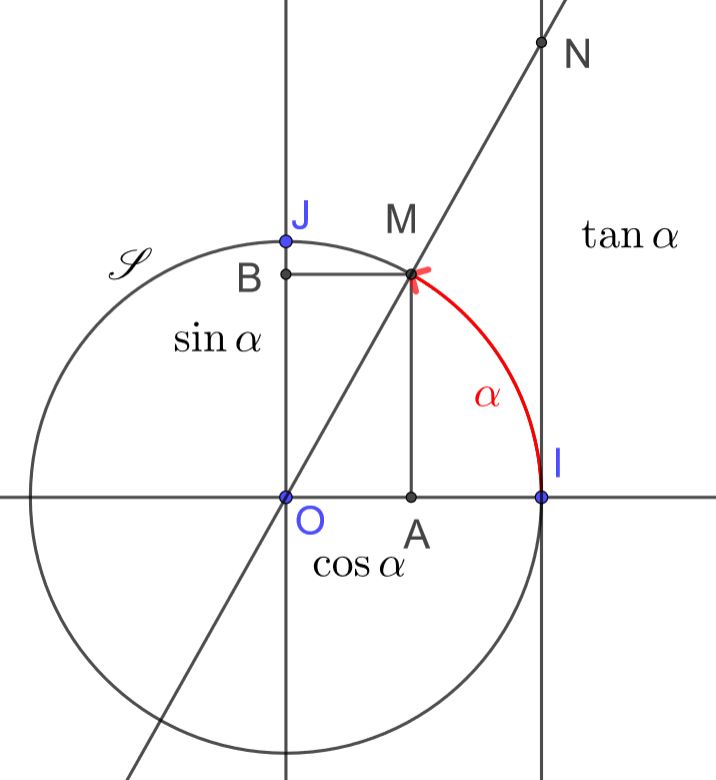
\includegraphics[width=0.4\textwidth]{image/fct_trigo/tangente.png}
			\caption{Construction géométrique de la tangente. Ici, $0<\alpha<\frac{\pi}{2}$, $OA=\cos\alpha$, $OB=BM=\sin\alpha$, $IN=\tan\alpha$.}
			\label{fig_tangente}
		\end{figure}

		\paragraph{Remarque.} De même que pour les fonctions cosinus et sinus, la définition de la fonction tangente s'étend sur $\R-\left\{\frac{\pi}{2}+k\Z\right\}$.

		\begin{thm}
			\begin{equation}
				\forall \alpha\in\R-\left\{\frac{\pi}{2}+k\Z\right\}, \tan\alpha=\frac{\sin\alpha}{\cos\alpha}.
			\end{equation}
		\end{thm}

		\begin{proof}
			On démontre le théorème dans le cas où $\alpha\in\[\left.0,\frac{\pi}{2}\right[\right.$, on laisse les autres cas au lecteur.
			Considérons la figure $\ref{fig_tangente}$. Par construction, $(IN)\sslash (AM)$, et on a $O\star A\star I$ et $O\star M\star N$. D'après le théorème de Thalès, on a 
			\begin{equation}
				\frac{IN}{AM}=\frac{OI}{OA} \label{eq_thales_trigo}
			\end{equation}
			Mais $IN=\tan\alpha$, $OI=1$, $OA=\cos\alpha$ et $AM=\sin\alpha$. Donc
			\begin{equation}
				\eqref{eq_thales_trigo}\Leftrightarrow \frac{\tan\alpha}{\sin\alpha}=\frac{1}{\cos\alpha}\Leftrightarrow\tan\alpha=\frac{\sin\alpha}{\cos\alpha}.
			\end{equation}
		\end{proof}

	\subsection{Exercices}
		\paragraph{Exercice 1.}
			Soit $\S$ le cercle trigonométrique dans un repère orthonormé direct $(O,I,J)$.
			\begin{enumerate}[1)]
				\item Placer un point $M$ sur $\S$, de coordonnées $(x,y)$, tel que $y=\frac{1}{2}$, et $x>0$. Combien vaut $\sin\widehat{IOM}$\,?
				\item Calculer $\cos\widehat{IOM}$. Calculer $\tan\widehat{IOM}$.
				\item Placer $N\in\S$, de coordonnées $(x',y')$, tel que $x'=\frac{1}{2}$ et $y'>0$.
				\item Remarquer une symétrie, et sans aucun calcul, en déduire les valeurs de $\cos\widehat{ION}$ et $\sin\widehat{ION}$.
			\end{enumerate}

		\paragraph{Exercice 2.}
			\begin{enumerate}[1)]
				\item Démontrer que $\forall x\in\R$, $\cos^2x+\sin^2x=1$.
				\item Soit $x\in\R$. Calculer les nombres suivants en fonction de $\cos x$ et $\sin x$\,:
				\begin{equation}
					\cos(-x);\quad \sin(-x);\quad \cos(\pi+x);\quad \sin(\pi+x);\quad \cos(\pi-x);\quad \sin(\pi-x); \nonumber
				\end{equation}
				\begin{equation}
					\quad\cos\(\frac{\pi}{2}+x\);\quad\sin\(\frac{\pi}{2}+x\);\quad\cos\(\frac{\pi}{2}-x\);\quad\sin\(\frac{\pi}{2}-x\);\quad\nonumber
				\end{equation}
				On pourra s'aider avantageusement d'un schéma du cercle trigonométrique et de considérations sur des symétries axiales et rotatives.
			\end{enumerate}


	\subsection{Trigonométrie dans le triangle rectangle}

		Dans tout triangle rectangle, les angles aux sommets sont compris entre 0 et $\frac{\pi}{2}$ et peuvent être considérés comme non orientés. 

		\begin{thm}
			Soit un triangle $ABC$ rectangle en $B$. Soit $\alpha=\widehat{BAC}$. Alors\,:
			\begin{equation}
				\cos\alpha=\frac{AB}{AC},
			\end{equation}
			\begin{equation}
				\sin\alpha=\frac{BC}{AC},
			\end{equation}
			\begin{equation}
				\tan\alpha=\frac{BC}{AB}.
			\end{equation}
			Par rapport au sommet $A$, on peut nommer les côtés\,: $[AC]$ étant l'hypothénuse du triangle rectangle, $[AB]$ est le côté adjacent (au sommet $A$), tandis que $[BC]$ est le côté opposé (au sommet $A$). On peut donc reformuler le théorème de manière \guil{mnémotechnique}\,:
			\begin{equation}
				\cos\alpha=\frac{\text{mesure du côté adjacent}}{\text{mesure de l'hypothénuse}}
			\end{equation}
			\begin{equation}
				\sin\alpha=\frac{\text{mesure du côté opposé}}{\text{mesure de l'hypothénuse}}
			\end{equation}
			\begin{equation}
				\tan\alpha=\frac{\text{mesure du côté opposé}}{\text{mesure du côté adjacent}}.
			\end{equation}
		\end{thm}

		\begin{figure}
			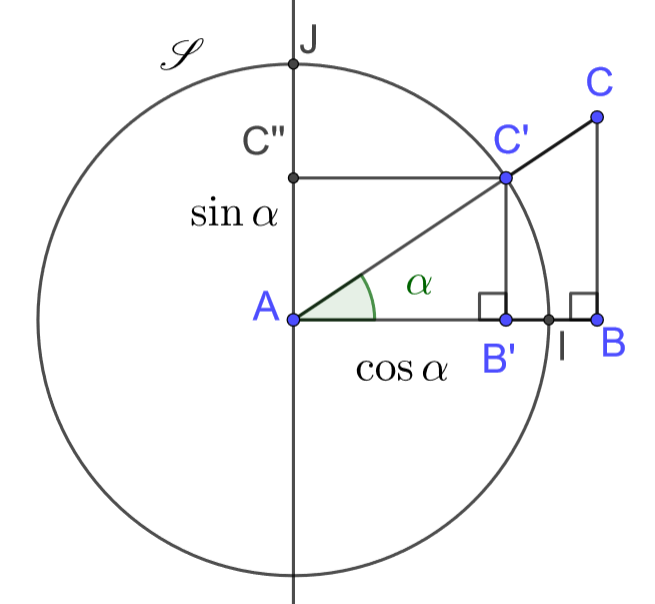
\includegraphics[width=0.4\textwidth]{image/fct_trigo/trigo_triangle.png}
			\caption{Figure pour passer d'un triangle rectangle au cercle trigonométrique. On a pris le cas où $AC>1$.}
			\label{fig_trigo_triangle}
		\end{figure}

		\begin{proof}
			On suppose que $\ovr{(A,B,C)}>0$ (le cas contraire se démontre de manière similaire, on laisse donc cela au lecteur). Construisons un cercle trigonométrique $\S$ de centre $A$, et posons $I=(AB)\cap\S$, et soit $J$ tel que $(A,I,J)$ soit un repère orthnormé direct. Soit $C'=(AC)\cup\S$. Soient $B'$ et $C''$ respectivement les projetés orthogonaux de $M$ sur $(OI)$ et sur $(OJ)$ (voir figure \ref{fig_trigo_triangle}). Alors $AB'=\cos\alpha$ et $B'C'=\sin\alpha$. Si $AC=1$, alors $C'=C$, $B'=B$, $BC=B'C'$ et les relations annoncées du théorème sont immédiatement vérifiées. Supposons que $AC>1$. Alors $A\star B'\star B$ et $A\star C'\star C$ (dans le cas contraire, on aurait $A\star B\star B'$ et $A\star C\star C'$). D'après le théorème de Thalès --- et ce, que $AC>1$ ou que $AC<1$ --- on a\,:
			\begin{equation}
				\frac{AB'}{AB}=\frac{AC'}{AC}=\frac{BC'}{BC}. \label{eq_thales_trigotriangle}
			\end{equation} 
			Mais dans le cercle trigonométrique, $\cos\alpha=AB'$, $AC'=1$ et $\sin\alpha=B'C'$. Ainsi, d'après \eqref{eq_thales_trigotriangle},
			\begin{equation}
				\frac{\cos\alpha}{AB}=\frac{1}{AC},\quad \text{donc}\quad \cos\alpha=\frac{AB}{AC}.
			\end{equation}
			De même, d'après \eqref{eq_thales_trigotriangle},
			\begin{equation}
				\frac{\sin\alpha}{BC}=\frac{1}{AC}\quad \text{donc}\quad \sin\alpha=\frac{BC}{AC}.
			\end{equation}
			Enfin,
			\begin{equation}
				\tan\alpha=\frac{\sin\alpha}{\cos\alpha}=\frac{\frac{AB}{AC}}{\frac{BC}{AC}}=\frac{AB}{AC}\cdot\frac{AC}{BC}=\frac{AB}{BC}.
			\end{equation}
		\end{proof}

		\paragraph{Exercice 1} Considérons un triangle $ABC$ rectangle en $B$, avec $AB=3$, $BC=4$.
		\begin{enumerate}[1)]
			\item Calculer $AC$.
			\item On pose $\alpha=\widehat{CAB}$, $\beta=\widehat{ABC}$. Calculer $\cos\alpha$, $\sin\alpha$, $\tan\alpha$. En déduire $\cos\beta$, $\sin\beta$, $\tan\beta$.
		\end{enumerate}

		\paragraph{Exercice 2} 		Aujourd'hui, les programmes de calculs (par exemple dans les calculatrices) permettent de calculer les valeurs des fonctions trigonométriques, des angles étant donnés. En attendant de voir comment les calculer, nous allons utiliser ces valeurs pour calculer des distances.
		
		Considérons un triangle $DEF$ rectangle en $E$ avec $DE=3$, et $\alpha=\widehat{FDE}=\frac{\pi}{6}$.
		\begin{enumerate}[1)]
			\item Utiliser une machine à calculer pour estimer numériquement la valeur de $\tan\(\frac{\pi}{6}\)$.
			\item Exprimer $\tan\alpha$ en fonction de $DF$ et $FE$.
			\item En déduire la valeur exacte, puis approchée, de la distance $FE$.
			\item En procédant de même avec l'aide de la fonction $\cos$, sans utiliser le théorème de Pythagore, calculer la distance $DE$.
		\end{enumerate}

		\paragraph{Exercice 3} Valeurs trigonométriques remarquables.
			Nous allons voir comment calculer certaines valeurs des fonctions trigonométriques (notamment $\pi/6$ utilisée précédemment).
			\begin{enumerate}[1)]
				\item $\pi/3$ et $\pi/6$. On considère un triangle équilatéral $ABC$. Pour simplifier, on prendra $AB=1$.
				\begin{enumerate}[a)]
					\item Justifier que $\widehat{CAB}=\pi/3$.
					\item Soit $H\in(AC)$ tel que $(BH)$ soit un axe de symétrie de la figure. Calculer $AH$ et $\widehat{HBA}$.
					\item Calculer $HB$.
					\item En considérant les bons angles, calculer exactement\,:
					\begin{equation}
						\cos{\frac{\pi}{6}},\quad \sin\frac{\pi}{6},\quad \cos{\frac{\pi}{3}},\quad \sin\frac{\pi}{3},\quad \tan{\frac{\pi}{6}},\quad \tan\frac{\pi}{3}.\nonumber
					\end{equation}
					Si besoin, vérifier les valeurs approchées avec une machine à calculer.
				\end{enumerate}
				\item $\pi/4$. Soit $DEF$ un triangle rectangle isocèle en $E$. Pour simplifier, on prendra $DF=1$.
				\begin{enumerate}[a)]
					\item Justifier que $\widehat{EDF}=\widehat{DFE}=\frac{\pi}{4}$.
					\item Démontrer que $\cos\frac{\pi}{4}=\sin\frac{\pi}{4}$. Calculer ces valeurs.
					\item Calculer $\tan\frac{\pi}{4}$.
					\item Si besoin, tout vérifier à la calculatrice.
				\end{enumerate}
			\end{enumerate}

			\emph{Solution : on peut résumer quelques valeurs particulières des fonctions trigonométriques dans le tableau suivant\,:}

			\renewcommand*{\arraystretch}{1.4}
			\begin{tabular}{cccccc}
				$\alpha$     & 0 & $\frac{\pi}{6}$     & $\frac{\pi}{4}$      & $\frac{\pi}{3}$      & $\frac{\pi}{2}$ \\
				\hline
				$\sin\alpha$ & 0 & $\frac{1}{2}$       & $\frac{\sqrt{2}}{2}$ & $\frac{\sqrt{3}}{2}$ & 1 \\
				$\cos\alpha$ & 1 & $\frac{\sqrt{3}}{2}$& $\frac{\sqrt{2}}{2}$ & $\frac{1}{2}$        & 0 \\
				$\tan\alpha$ & 0 & $\frac{\sqrt{3}}{3}$& 1                    & $\sqrt{3}$           & non défini
			\end{tabular}

		\paragraph{Exercice 4} (Géométrie sphérique sur la Terre)

			La surface de la Terre est modélisée par une sphère de rayon $R=CE=CM=CN=CS\approx 6400$km. Les \emph{parallèles} sont des cercles inscrits sur la sphère, perpendiculaires à l'axe Nord-Sud $(NS)$. L'équateur est le parallèle qui divise la Terre en deux hémisphères symétriques. Le 40$^\e$ parallèle Nord est l'ensemble des points de l'hémisphère Nord qui sont à une lattitude de 40$^\circ$. En particulier, $ECM=40^\circ$.
			
			\vspace{0.4cm}

			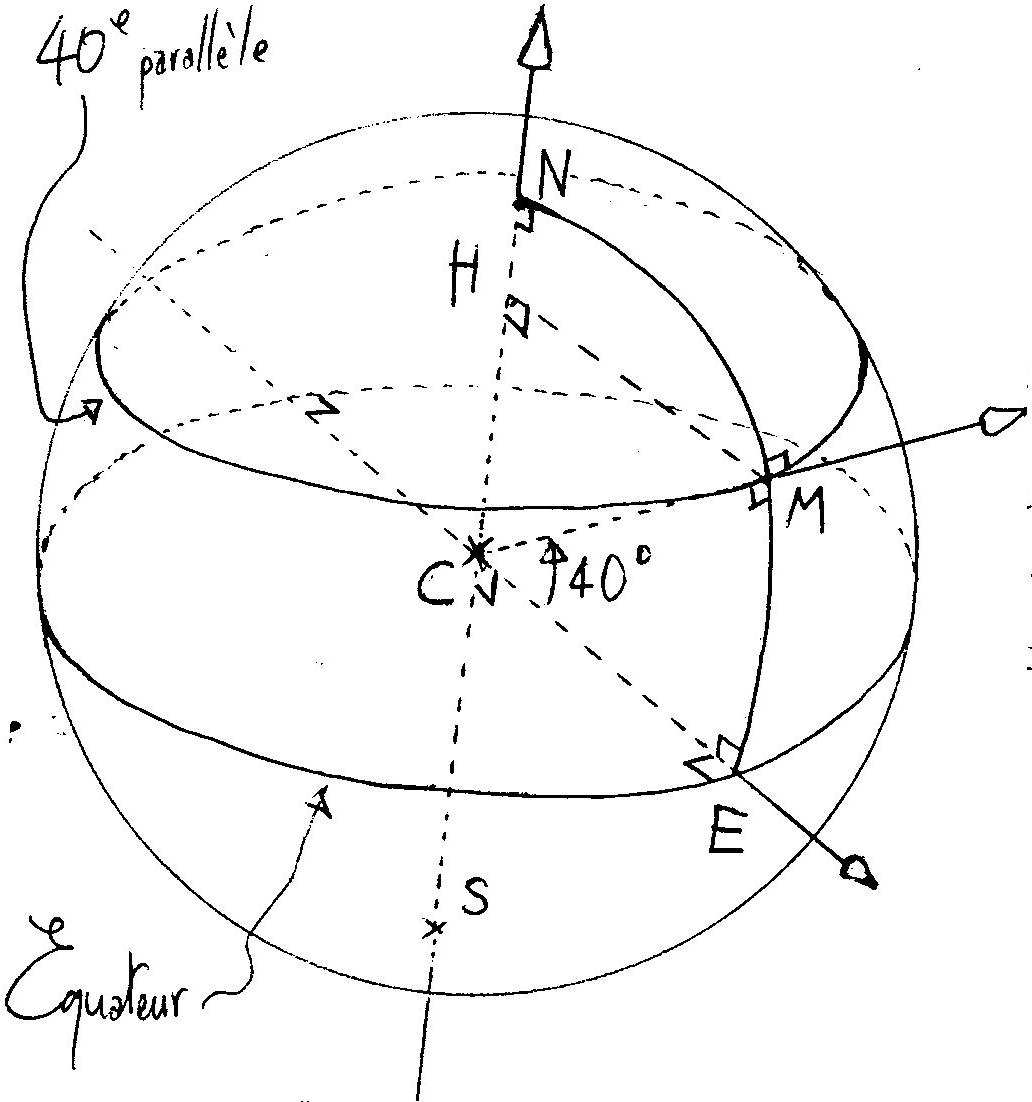
\includegraphics[width=0.6\textwidth]{image/fct_trigo/exo_trigo_sphere.jpg}
			
			\begin{enumerate}[1)]
				\item En sachant que $[HM]$ est un rayon du 40$^\e$ parallèle, calculer la longueur de ce parallèle à 100km près.
				\item Calculer la longueur du $x^\e$ parallèle en fonction de $x$ et de $R$. 
			\end{enumerate}


	\subsection{Formulaire de trigonométrie}
		\paragraph{Exercice } (Formules de trigonométrie)

		On étudie des manipulations algébriques fort utiles pour calculer les fonctions trigonométriques de valeurs particulières, ainsi que pour les problèmes physiques. On commence par exprimer les fonctions trigonométriques de la somme de deux angles, mettons $\alpha+\beta$, en fonction de $\sin\alpha$, $\sin\beta$, $\cos\alpha$ et $\sin\beta$ seulement. Même si la relation sera vraie pour tous angles orientés $\alpha$ et $\beta$ appartenant à $\R$, on effectue une preuve pour des angles orientés positifs tels que $\alpha+\beta<\frac{\pi}{2}$. L'extension de cette démonstration dans les autres cas est laissée au lecteur. On considère donc la figure \ref{fig_sin_add}.

		\begin{figure}
			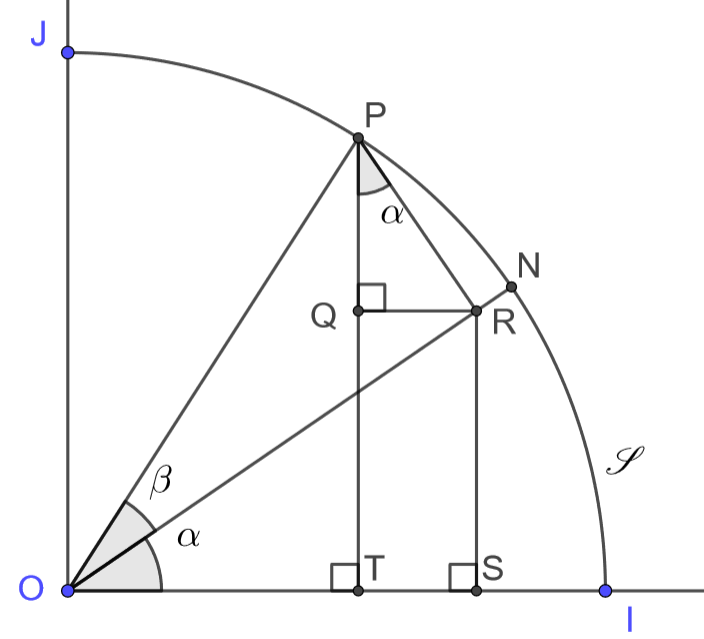
\includegraphics[width=0.5\textwidth]{image/fct_trigo/sin_addition.png} 
			\caption{Un cas particulier d'addition d'angles.}
			\label{fig_sin_add}
		\end{figure}
		

	\begin{enumerate}
		\item Calcul de $\sin(\alpha+\beta)$.
		\begin{enumerate}[a.]
			\item Vérifier rapidement que\,:
			\begin{equation}
			 	\sin(\alpha+\beta)=PQ+RS,\quad \sin\beta=PR,\quad \cos\beta=OR.
			\end{equation} 
			\item Démontrer que, comme indiqué sur la figure, $\widehat{QPR}=\alpha$, et en déduire que $\sin\alpha=\frac{RS}{OR}$.
			\item Exprimer $PQ$ et $PR$ en fonction de $\cos\alpha$, $\sin\alpha$, $\cos\beta$, $\sin\beta$.
			\item Conclure\,: exprimer $\sin(\alpha+\beta)$ en fonction de $\cos\alpha$, $\sin\alpha$, $\cos\beta$, $\sin\beta$.
		\end{enumerate}
		\item Extensions immédiates. Pour cette question, on utilisera abondamment les résultats de l'exercice 2 de la section \ref{subsec_sincos}.
		\begin{enumerate}[a.]
			\item En transformant $b$ en $-b$, calculer $\sin(\alpha-\beta)$ en fonction de $\cos\alpha$, $\sin\alpha$, $\cos\beta$, $\sin\beta$.
			\item En transformant $a$ en $\psd-a$, $b$ en $-b$, calculer $\cos(\alpha+\beta)$ en fonction de $\cos\alpha$, $\sin\alpha$, $\cos\beta$, $\sin\beta$.
			\item De même qu'en a., en déduire $\cos(\alpha-\beta)$.
		\end{enumerate}
		\item Formules de duplication, et de l'angle de moitié.
		\begin{enumerate}[a.]
			\item En considérant le cas où $\alpha=\beta$, calculer $\sin(2\alpha)$  en fonction de $\cos\alpha$ et $\sin\beta$.
			\item De même, calculer $\cos(2\alpha)$ en fonction de  $\cos\alpha$ et $\sin\beta$. En se souvenant que $\cos^2\alpha+\sin^2\alpha=1$, en déduire $\cos(2\alpha)$ en fonction de $\sin\alpha$ seulement, puis de $\cos\alpha$ seulement.
			\item Secouer les équations pour exprimer $\sin^2\alpha$ en fonction de $\cos(2\alpha)$, puis $\cos^2\alpha$ en fonction de $\cos(2\alpha)$
		\end{enumerate}
	\end{enumerate}

	\emph{Solutions} On donne les solutions sous la forme d'un formulaire de trigonométrie (circulaire). Certaines formules ne font pas partie de l'exercice, mais nous invitons tout de même le lecteur à les démontrer. $a$, $b$, $p$, $q$, sont des nombres réels, sauf dans les cas où ils compromettraient la définition d'une tangente ou d'un nombre avec dénominateur, auquel cas on laisse le lecteur adapter les définitions.

	\emph{Formules quadratiques}
	\begin{equation}
		\cos^2a+\sin^2a=1,\quad 1+\tan^2a=\frac{1}{\cos^2a}.
	\end{equation}
	\emph{Formules d'addition}
	\begin{equation}
		\cos(a+b)=\cos a\cos b -\sin a\sin b,\quad \sin(a+b)=\sin a \cos b + \sin b \cos a,
	\end{equation}
	\begin{equation}
		\cos(a-b)=\cos a \cos b + \sin a \sin b,\quad \sin(a-b)=\sin a \cos b - \sin b \cos a.
	\end{equation}
	\begin{equation}
		\tan(a+b)=\frac{\tan a+\tan b}{1-\tan a\tan b},\quad \tan(a-b)=\frac{\tan a-\tan b}{1+\tan a\tan b}
	\end{equation}
	\emph{Formules de duplication et de linéarisation}
	\begin{equation}
		\cos 2a = \cos^2a-\sin^2a=2\cos^2a-1=1-2\sin^2a,\quad 	\sin 2a=2\sin a \cos a,
	\end{equation}
	\begin{equation}
		\cos^2a=\frac{1}{2}+\frac{\cos a}{2},\quad \sin^2a=\frac{1}{2}-\frac{\cos 2a}{2}
	\end{equation}
	\begin{equation}
		\tan 2a=\frac{2\tan a}{1-\tan^2a}
	\end{equation}
	\emph{Formules du produit}
	\begin{equation}
		\cos a\cos b=\frac{1}{2}(\cos(a-b)+\cos(a+b)),\quad \cos a \sin b=\frac{1}{2}(\sin(a+b)-\sin(a-b)),
	\end{equation}
	\begin{equation}
		\sin a\sin b=\frac{1}{2}(\cos(a-b)-\cos(a+b)),
	\end{equation}
	\begin{equation}
		\cos p+\cos q=2\cos\frac{p+q}{2}\cos\frac{p-q}{2},\quad \cos p-\cos q=-2\sin\frac{p+q}{2}\sin\frac{p-q}{2},
	\end{equation}
	\begin{equation}
		\sin p +\sin q=2\sin\frac{p+q}{2}\cos\frac{p-q}{2},\quad \sin p -\sin q=2\sin\frac{p-q}{2}\cos\frac{p+q}{2}.
	\end{equation}
	\emph{Formules de la tangente de l'angle de moitié}
	On pose $t=\tan\frac{a}{2}$. Alors\,:
	\begin{equation}
		\cos a=\frac{1-t^2}{1+t^2}\quad \sin a=\frac{2t}{1+t^2},\quad \tan a=\frac{2t}{1-t^2}.
	\end{equation}
\paragraph{Application\,: valeurs numériques des fonctions trigonométriques.}
En utilisant ces formules de trigonométrie, on peut fabriquer des tables qui contiennent les valeurs des fonctions trigonométriques, uniquement à partir des valeurs remarquables calculées plus haut. Nous savons par exemple que $\cos\frac{\pi}{4}=\frac{\sqrt{2}}{2}$. De là, à partir de la formule de duplication, on calcule directement que
\begin{equation}
    \cos\frac{\pi}{8}=\sqrt{\frac{\cos\frac{\pi}{4}+1}{2}}=\sqrt{\frac{\frac{\sqrt{2}}{2}+1}{2}}.\nonumber
\end{equation}
Puis,
\begin{equation}
    \cos{\frac{\pi}{16}}=\sqrt{\frac{\cos\frac{\pi}{8}+1}{2}}=\sqrt{\frac{\sqrt{\frac{\frac{\sqrt{2}}{2}+1}{2}}+1}{2}}.\nonumber
\end{equation}
Bref, on peut montrer facilement que
\begin{equation*}
    \forall n\in\N, \cos\frac{\pi}{4\cdot 2^{n+1}}=\sqrt{\frac{\cos\frac{\pi}{4\cdot 2^n}+1}{2}}.
\end{equation*}
Et de même,
\begin{equation*}
    \forall n\in\N, \sin\frac{\pi}{4\cdot 2^{n+1}}=\sqrt{1-\frac{\cos\frac{\pi}{4\cdot 2^n}}{2}}.
\end{equation*}
Cela nous permet en principe de calculer les valeurs du cosinus de nombres aussi petits que l'on veut. Ensuite, si l'on cherche la valeur du cosinus d'un nombre $x\in\[0,\psd\]$, on peut approcher la valeur de $x$ à $\varepsilon$ près en choisissant un nombre $n$ tel que $\frac{\pi}{4\cdot 2^n}<\varepsilon$, et un nombre $k$ tel que $k\frac{\pi}{4\cdot 2^n}<x<(k+1)\frac{\pi}{4\cdot 2^n}$. En utilisant $k-1$ fois la formule d'addition pour le cosinus, à partir des valeurs de $\cos\frac{\pi}{4\cdot 2^n}$ et $\sin\frac{\pi}{4\cdot 2^n}$, on peut trouver les valeurs de $\cos \(k\frac{\pi}{4\cdot 2^n}\)\approx\cos x$ et de $\sin\(k\frac{\pi}{4\cdot 2^n}\)\approx \sin x$. En effet,
\begin{equation*}
    \cos\(k\frac{\pi}{4\cdot 2^n}\)=\cos\(\frac{\pi}{4\cdot 2^n}+\ldots+\frac{\pi}{4\cdot 2^n}\)
\end{equation*}
où il y a $k-1$ additions, et de même pour $\sin\(k\frac{\pi}{4\cdot 2^n}\)$.

On peut donc approcher toute valeur des fonctions trigonométriques avec des expressions qui ne font intervenir que des racines carrées. 

\paragraph{Approcher la valeur du nombre \pi}

C'est pour cette raison que la formule parachutée à la fin du chapitre \ref{chap_pinombre} (équation \eqref{eq_serpent}) n'était pas si \guil{circulaire} que cela. En effet, nous avions montré que 
\begin{equation*}
    \pi=\lim\limits_{n\to\infty}n\sin\(\frac{\pi}{n}\).
\end{equation*}
Mais en remplaçant $n$ par $4\cdot 2^n$, cette égalité devient

\begin{equation*}
    \pi=\lim\limits_{n\to\infty}4\cdot 2^n\sin\(\frac{\pi}{4\cdot 2^n}\).
\end{equation*}
Et nous avons alors un processus qui permet d'approcher la valeur du nombre $\pi$. En fait, si l'on déroule les calculs (exercice\,: le faire\,!), on trouvera des formules très similaires à celles du chapitre \ref{chap_pinombre}.


\section{Fonctions trigonométriques réciproques.}

	\subsection{Résolution d'équations trigonométriques}
		\begin{thm}
			Soient $u,v\in\R$. Alors\,:
			\begin{equation}
				\sin u=\sin v\Leftrightarrow ((u\equiv v[2\pi])\lor(u\equiv\pi-v[2\pi])),
			\end{equation}
			\begin{equation}
				\cos u=\cos w\Leftrightarrow ((u\equiv w[2\pi])\lor(u\equiv-w[2\pi])).
			\end{equation}
		\end{thm}
		\emph{Idée de preuve.} Pour démontrer ce théorème, il faudrait d'abord parler de continuité et de construction rigoureuse de nombres réels. Cela sera fait dans une prochaine session. On peut cependant donner une idée intuitive de la preuve en s'aidant des schémas suivants. Considérons un angle $u$ repéré sur le cercle trigonométrique et demandons-nous quels autres angles peuvent donner des sinus et des cosinus égaux. Sur la figure \ref{fig_egal_angles_trigo}, on voit que\footnote{Tout mathématicien rigoureux doit se méfier d'arguments tels que \guil{on voit que}\,!} l'angle $v=\pi-u$ égalise les sinus, tandis que l'angle $w=-u$ égalise les cosinus. Et bien sûr, il faut se rappeler que cela se fait à des tours complets près, d'où le modulo $2\pi$.

		\begin{figure}
			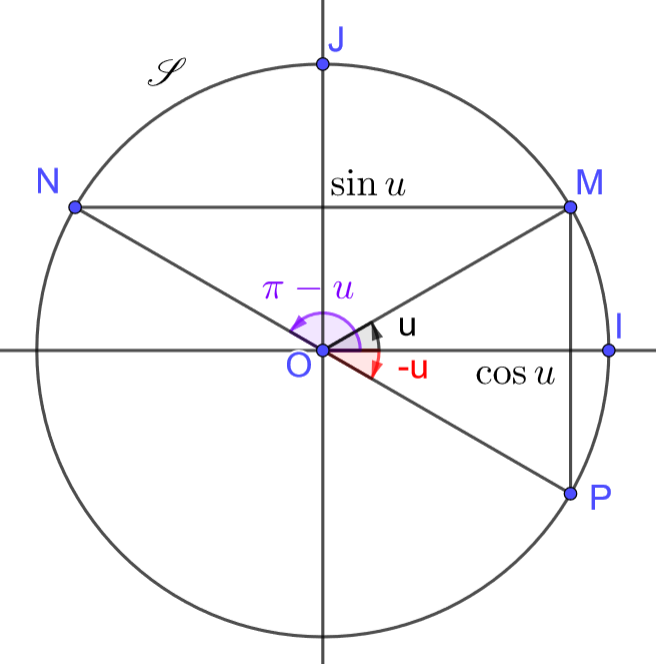
\includegraphics[width=0.5\textwidth]{image/fct_trigo/resol_eq_trigo.png}
			\caption{Résolution graphique d'équation trigonométrique. Ici, on a pris le cas où $0<u<\psd$. Nous invitons le lecteur à tracer les schémas des autres cas.}
			\label{fig_egal_angles_trigo}
		\end{figure}

		\paragraph{Exercice.} En s'aidant d'un tracer du cercle trigonométrique, résoudre les équations suivantes\,:
		\begin{equation}
			\cos x=\frac{\sqrt{3}}{2},\quad \sin x=-\frac{1}{2},\quad \cos 2x=\frac{\sqrt{2}}{2}.
		\end{equation}

		\emph{Solutions\,:}
		\begin{equation}
			\cos x=\frac{\sqrt{3}}{2}\Leftrightarrow x\equiv\pm\frac{\pi}{6}[2\pi],\quad\sin x=-\frac{1}{2}\Leftrightarrow\(x\equiv-\frac{\pi}{6}[2\pi]\lor x\equiv -\frac{5\pi}{6}[2\pi]\),
		\end{equation}
		\begin{equation}
			\cos 2x=\frac{\sqrt{2}}{2}\Leftrightarrow x\equiv\pm\frac{\pi}{8}[\pi].
		\end{equation}


	\subsection{Fonctions trigonométriques réciproques}
		\begin{thm}
			Soit $y\in[-1,1]$. Alors il existe un unique nombre réel $u$ dans l'intervalle $[0,\pi]$ tel que $y=\cos u$, et il existe un unique nombre réel $v$ dans l'intervalle $[-\pi,\pi]$ tel que $y=\cos v$. Par définition, on pose\,:
			\begin{equation}
				u=\acos y, \quad v=\asin y;
			\end{equation}
			$\acos$ est la fonction \emph{arc cosinus}, et $\asin$ est la fonction \emph{arc sinus}.

			Soit $z\in\R$. Alors il existe un unique nombre réel $w$ dans l'intervalle $\left]-\frac{\pi}{2},\frac{\pi}{2}\right[$, tel que $z=\tan w$. Par définition, on pose\,:
			\begin{equation}
				w=\atan z;
			\end{equation}
			$\atan$ est la fonction \emph{arc tangente}.
		\end{thm}

		La démonstration rigoureuse de ce théorème demande d'utiliser la notion de continuité des fonctions, qui sera vue dans la prochaine session de cours. Même si je dois vous demander de l'admettre, on peut quand même se convaincre \guil{visuellement} du résultat. En effet, en visualisant le cercle trigonométrique, si l'on contraint l'angle $u$ orienté à balayer l'intervalle $\[-\psd,\psd\]$, tout nombre $y$ compris entre $-1$ et $1$ sera atteint par $\sin u$ une et une unique fois, et si l'angle $v$ balaye l'intervalle $[0,2\pi]$, alors ce nombre $y$ sera atteint une et une unique fois par $\cos v$. Lorsque $w$ balaye l'intervalle $\left]-\psd,\psd\right[$, $\tan w$ balaye l'ensemble des nombres réels. On peut s'en convaincre en constatant que plus $w$ se rapproche de $-\psd$ sans jamais l'atteindre, plus $\tan w$ prend de grandes valeurs négatives, jusqu'à tendre vers $-\infty$\,; de même, lorsque $w$ se rapproche de $\psd$, $\tan w$ tend vers $+\infty$. Comme le nombre $\tan w$ ne fait que croître avec $w$, on peut comprendre intuitivement que tout nombre réel est atteint une et une unique fois par $\tan w$ lorsque $w$ balaye l'intervalle $\left]-\psd,\psd\right[$.

	\subsection{Représentation graphique des fonctions trigonométriques}
		Les fonctions $\sin$ et $\cos$ sont définies sur $\R$, il est possible de tracer leur graphe. On a déjà un début de tableau de valeurs, mais en plus, on sait qu'à chaque fois que l'argument de ces fonctions avance de $2\pi$, la fonction devient identique à elle-même. Autrement dit, $\forall x\in\R, \cos(x+2\pi)=\cos x, \sin(x+2\pi)=\sin x$. On n'a donc besoin de tracer ces fonctions que sur un intervalle de longueur $2\pi$, puis il suffit de reproduire le graphe à l'identique. Dans la figure \ref{fig_graphefcttrig}, on a représenté les graphes des fonctions $\cos$ et $\sin$.

		\begin{figure}
			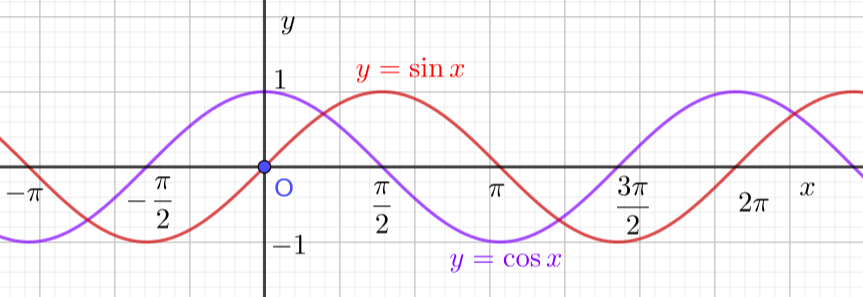
\includegraphics[width=0.8\textwidth]{image/fct_trigo/courbes_trigo.png}
			\caption{Représentation graphique des fonctions trigonométriques.}
			\label{fig_graphefcttrig}
		\end{figure}

		La fonction tangente a quelqu'originalité en plus, puisqu'elle diverge à chaque fois que l'on atteint $\pm\psd[\pi]$. Elle est définie sur $\R-\left\{\psd+k\pi,k\in\Z\right\}$, ou de manière plus synthétique, $\R-\left\{\psd+\pi\Z\right\}$. Sa courbe est représentée figure \ref{fig_plot_tan}.

		\begin{figure}
			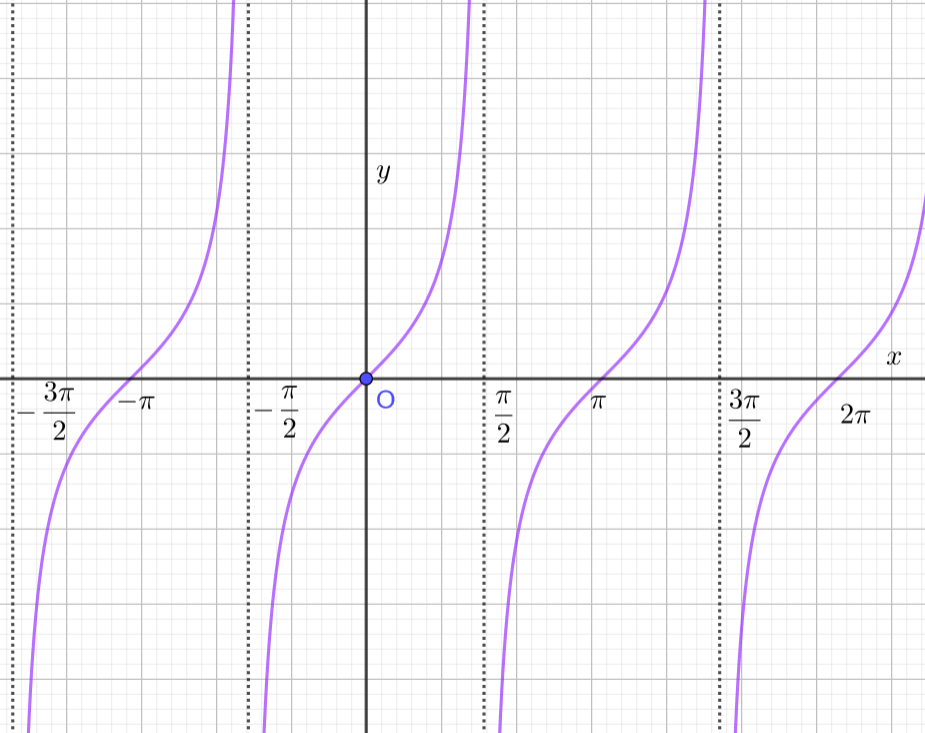
\includegraphics[width=0.8\textwidth]{image/fct_trigo/plot_tan.png}
			\caption{Représentation graphique de la fonction tangente. On a représenté en pointillé les lignes qui correspondent aux valeurs interdites, c'est-à-dire $\psd[\pi]$. On peut visualiser aisément les comportement \guil{infinis} au voisinage de ces points.}
			\label{fig_plot_tan}
		\end{figure}

		Le théorème suivant permet de tracer les fonctions réciproques. Nous en donnons l'illustration figures $\ref{fig_asincos}-\ref{fig_atan}$.

		\begin{thm}
			\begin{itemize}[label=\textbullet]
				\item Le graphe de la fonction $\asin$ est le symétrique du graphe de la fonction $\sin$ restreinte à l'intervalle $\[-\psd,\psd\]$, par rapport à la droite d'équation $y=x$.
				\item Le graphe de la fonction $\acos$ est le symétrique du graphe de la fonction $\cos$ restreinte à l'intervalle $[0,2\pi]$. 
				\item Le graphe de la fonction $\atan$ est le symétrique du graphe de la fonction $\tan$ restreinte à l'intervalle $\left]-\psd,\psd\right[$.
			\end{itemize}
			  
		\end{thm}
		\begin{proof}
			On ne démontre que le premier point, les autres s'effectuent de manière similaire. Considérons $\Gamma$ le graphe de la fonction $\sin$ restreinte à l'intervalle $\[-\psd,\psd\]$.  Pour tout $x\in\[-\psd,\psd\]$, le point de coordonnées $(x,\sin x)$ est sur ce graphe. Ceci étant donné, pour construire le graphe de la fonction $\asin$, il suffit d'inverser l'ordre des coordonnées, puisque cette fonction a pour objet de transformer $y=\sin x$ en $x=\acos y$. En effet, soit $y\in [0,1]$. Il existe un unique $x\in\[-\psd,\psd\]$ tel que $\sin x=y$, et on a $y=\asin x$. Donc le point de coordonnée $(x,y)$ appartient à $\Gamma$, et le point de la courbe souhaitée s'obtient par inversion de l'ordre des coordonnées, et donc, par symétrie d'axe $(d)$ où $(d)$ a pour équation $y=x$. 

			Les autres graphes se construisent de manière similaire. En fait, toute fonction réciproque se trace par symétrie autour de $(d)$. 
		\end{proof}


		\begin{figure}
			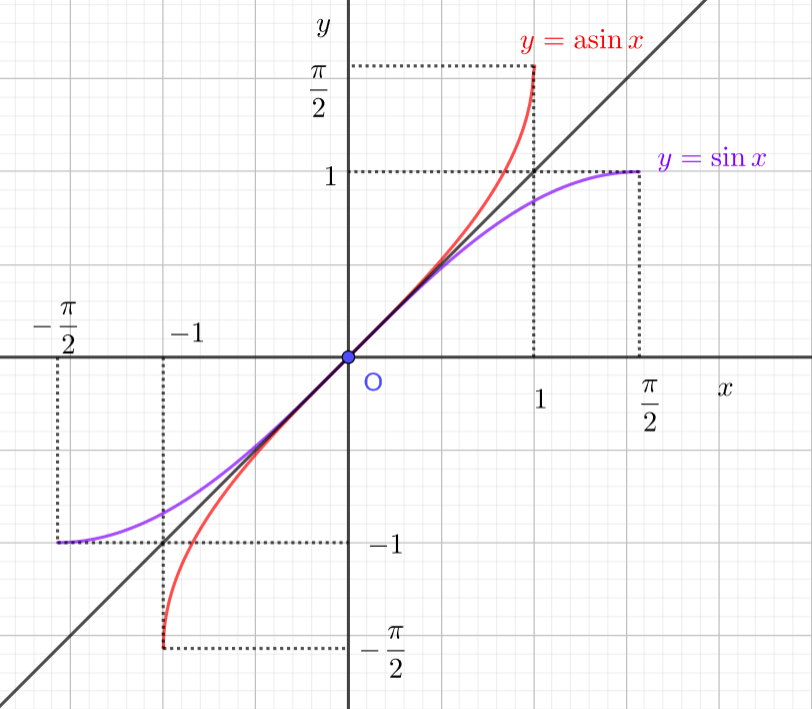
\includegraphics[width=0.55\textwidth]{image/fct_trigo/courbe_asin.png} 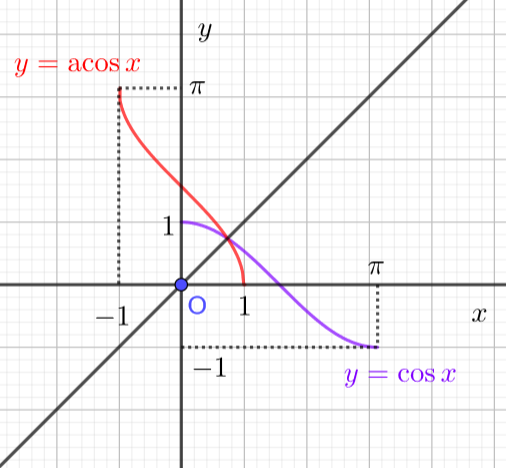
\includegraphics[width=0.43\textwidth]{image/fct_trigo/courbe_acos.png}
			\caption{À gauche\,: graphe de la fonction $\asin$ construit à partir de celui de $\sin$. À droite\,: idem pour $\acos$ et $\cos$.}
			\label{fig_asincos}
		\end{figure}
		\begin{figure}
			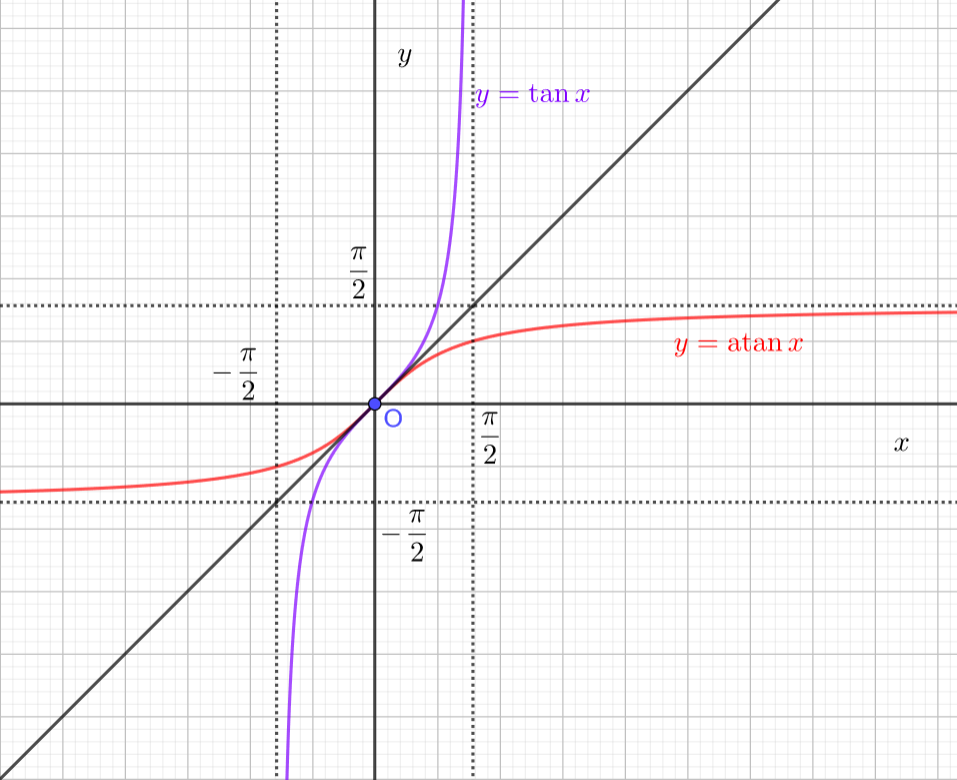
\includegraphics[width=0.8\textwidth]{image/fct_trigo/courbe_atan.png}
			\caption{Représentation graphique de la fonction $\atan$ à partir de celui de $\tan$.}
			\label{fig_atan}
		\end{figure}

		\vspace{0.3cm}

		Les fonctions trigonométriques réciproques permettent de calculer des angles, lorsque l'on connaît uniquement leurs cosinus et sinus. C'est ainsi que lorsque vous étiez petits, on vous demandait de calculer les angles d'un triangle rectangle dont les mesures des côtés étaient données. Considérons un triangle $ABC$ rectangle en $B$, mettons que l'on connaisse deux grandeurs, par exemple $AB=a$, $AC=b$ (on pourrait déduire la troisième via le théorème de Pythagore, mais peu importe). Alors, puisque $\cos\widehat{BAC}=\frac{AB}{AC}=\frac{a}{b}$, on a directement $\widehat{BAC}=\acos\(\frac{a}{b}\)$. Si l'on ne connaissait que $AB=a$ et $BC=c$, alors puisque $\tan\widehat{BAC}=\frac{BC}{AB}=\frac{c}{a}$, on déduit également que $\widehat{BAC}=\atan\(\frac{c}{a}\)$. Et enfin, de même, on montre que $\widehat{BAC}=\asin\(\frac{c}{b}\)$. C'est la principale utilité des fonctions trigonométriques réciproques. Mais on peut également s'amuser à démontrer des relations algébriques\,:

		\paragraph{Exercice.} Démontrer que\,:
		\begin{enumerate}
			\item $\forall x\in\[0,1\], \acos x+\asin x=\psd$,
			\item $\forall x\in[-1,1], \cos(\asin x)=\sin(\acos x)=\sqrt{1-x^2}$,
			\item 
			\begin{equation}
				\forall x\in]-1,1[,\quad  \tan(\asin x)=\frac{x}{1-x^2},\quad\forall x\in]-1,1[-\{0\},\quad  \tan(\acos x) = \frac{\sqrt{1-x^2}}{x},
			\end{equation}
			\item 
			\begin{equation}
				\forall x\in\R,\quad \sin(\atan x)=\frac{x}{\sqrt{1+x^2}},\quad \cos(\atan x)=\frac{1}{\sqrt{1+x^2}}.
			\end{equation}
		\end{enumerate}
		 

		\noindent\emph{Solution.} 
		\begin{enumerate}
			\item Soit $x\in[0,1]$. $\exists ! \theta\in\[0,\psd\],x=\cos \theta$, et de plus, $\acos x = \theta$. Mais comme $\cos \theta=\sin\(\psd-\theta\)=x$, on a $\asin x=\psd-\theta=\psd-\acos x$. D'où le résultat.
			\item $\acos$ est une fonction positive comprise entre $0$ et $\pi$, donc $\forall x\in[-1,1], \sin(\acos x)\ge 0$. De là, il suffit d'écrire que $\cos^2(\acos x)+\sin^2(\acos x)=1=x^2+\sin^2(\acos x)$, d'où la deuxième égalité. La première se démontre de manière similaire.
			\item Il suffit d'écrire que $\tan(\asin x)=\frac{\sin(\asin x)}{\cos(\asin x)}$ et d'utiliser la question précédente. On procède de même pour la deuxième égalité.
			\item Considérons un triangle rectangle $ABC$ rectangle en $B$, notons $\alpha$ l'angle au sommet de $A$. Supposons que $AB=1$ et $BC=x>0$ (le cas $x<0$ se traite aisément en utilisant les propriétés des fonctions trigonométriques). Alors $AC=\sqrt{1+x^2}$, $\sin\alpha=\frac{x}{\sqrt{1+x^2}}$, mais $\tan\alpha=x/1=x$, donc $\alpha=\atan x$, d'où le résultat. On procède de même pour la deuxième égalité.
		\end{enumerate}
		
		

\section{Utilité de la trigonométrie en Mécanique}
La Mécanique est l'art d'étudier le mouvement des corps matériels. C'est une branche de la science physique, dont l'objet est d'étudier les rapports quantitatifs entre des grandeurs mesurables des corps matériels afin d'en extraire des lois universelles et univoques.

	\subsection{Mouvement de rotation uniforme et roulement sans glissement}
		On considère une roue de rayon $R$ qui a un mouvement de rotation constant, et qui effectue un tour complet pendant la durée $T$. Le centre et l'axe de la roue sont fixés. On nomme $O$ ce centre, et on considère un repère orthonormé $(O,I,J)$ fixe par rapport à un observateur (il ne suit pas le mouvement de rotation) dans le même plan que la roue. On note $t$ la date qu'affiche un chronomètre lancé à $t=0$. Par convention, si un point $M$ a un mouvement qui dépend de la variable temporelle $t$, on exprimera cette dépendance en utilisant les notations des fonctions, et on notera $M(t)$ la position du point $M$ à la date $t$.
		\begin{enumerate}
			\item Montrer qu'un point $M(t)$ à l'extrémité de la roue tel que $M(0)$ a pour coordonnées $(R,0)$, a pour coordonnées à la date $t$\,: $(R\cos\omega t, R\sin\omega t)$, où on exprimera $\omega$ en fonction de $t$.
			\item En calculant la distance que fait le point $M$ pendant la durée $T$, calculer sa vitesse.
			\item Désormais on suppose que la roue roule sur le sol sans glisser. Cela signifie que le mouvement d'ensemble de la roue est tel que sa vitesse $v$ compense exactement la vitesse à l'extrémité de la roue, de telle sorte que la différence de vitesse entre l'extrémité de la roue qui touche le sol, et le sol, est nulle.
			\begin{enumerate}[a.]
			 	\item En déduire une relation entre $v$ et $\omega$.
			 	\item Calculer les coordonnées du point $O$ en fonction de $t$, sachant que $O(0)=(0,R)$ (on suppose que le sol est représenté par l'axe des abscisses).
			 	\item Par conséquent, le point $M(t)$ est tel que $M(0)$ a pour coordonnées $(R,R)$. En ajoutant le mouvement d'ensemble selon l'axe des abscisses $(Ox)$, démontrer que les coordonnées de $M(t)$ sont $(R(\cos(\omega t)-\omega t), R\sin \omega t)$.
			\end{enumerate} 
		\end{enumerate}
		La trajectoire d'un tel point est communément appelée \guil{cycloïde}. On représente cela figure \ref{fig_cyclo}.

		\begin{figure}
			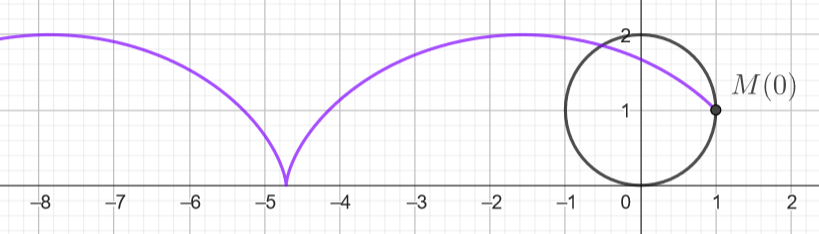
\includegraphics[width=0.6\textwidth]{image/fct_trigo/cyclo1.png}\\
			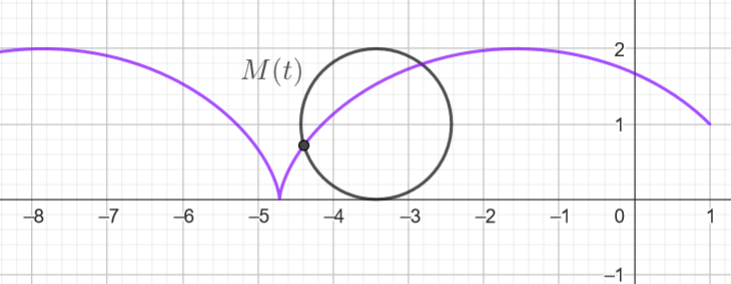
\includegraphics[width=0.6\textwidth]{image/fct_trigo/cyclo2.png}\\
			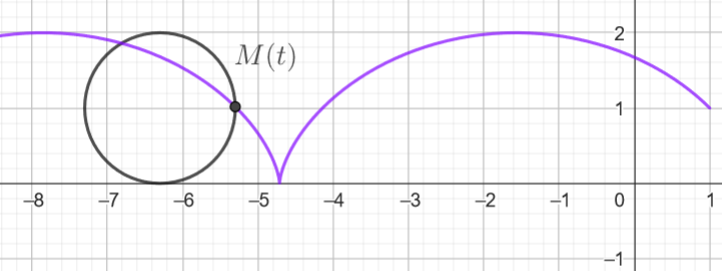
\includegraphics[width=0.6\textwidth]{image/fct_trigo/cyclo3.png}
			\caption{Représentation de la cycloïde et du cercle à trois instants. En haut\,: à $t=0$. En bas\,: à $t=\frac{2\pi}{\omega}$, la roue a réalisé un tour complet. Au milieu\,: date intermédiaire. On remarque que, puisque la roue tourne dans le sens trigonométrique, elle roule vers la gauche. On peut trouver moult animations de la cycloïde sur internet.}
			\label{fig_cyclo}
		\end{figure}

\iffalse
	\subsection{Loi de réfraction de Descartes}
		Tout le monde a fait l'expérience de l'illusion du bâton cassé lorsqu'il est plongé dans l'eau. Cela vient du fait que dans les milieux transparents, la lumière se propage plus lentement que dans le vide. Dans le vide, la célérité\footnote{En physique ondulatoire on préfère parler de célérité que de vitesse lorsqu'il s'agit de propagation d'une onde.} de la lumière vaut exactement $c=299\,792\,458$m/s. Dans un milieu $A$, la célérité de la lumière mesure $c_A<c$, et on défini l'indice de réfraction du milieu $A$ comme étant égal au rapport entre $c$ et $c_A$\,: $n_A=\frac{c}{c_A}$. Ainsi, l'indice de réfraction du vide vaut $1$ et tous les milieux transparents ont un indice de réfraction plus grand que $1$. Cette différence de vitesse de propagation implique des déviations de rayons lumineux. En physique ondulatoire, on peut démontrer que les trajectoires des rayons lumineux suivent ce que Fermat avait pris pour postulat\,:
		\begin{post}[Principe de Fermat]
			Lorsqu'un rayon lumineux peut relier deux points $A$ et $B$, il le fait en prenant le chemin optique qui minimise localement\footnote{Vu qu'il s'agit d'une minimisation locale, la lumière peut donc prendre plusieurs chemins. On verra quelques exemples plus bas.} la durée du parcours de la lumière\footnote{En vérité, une maximisation conviendrait aussi, mais dans presque tous les cas pratiques, il s'agit d'une minimisation.}
		\end{post}

		À présent considérons un miroir plan, un point $A$ et un point $B$. Bien sûr, la ligne droite qui relie $A$ et $B$ convient pour un rayon lumineux. Mais on sait que la lumière peut se réfléchis sur le miroir. Soit $M$ le point du miroir en lequel le rayon se réfléchit. On peut tracer $B'$, le symétrique de $B$ par rapport au plan du miroir. On a $AM+MB=AM+MB'$. Soit $M_0$ le point du miroir tel que $A$, $M_0$ et $B'$ soient alignés. Si le point $M$ est différent du point $M_0$, par inégalité triangulaire, le chemin réalisé sera plus long. Donc $M_0$ est le point solution. Par construction, on vérifie donc la loi suivante\,:
		\begin{thm}
			Lorsque la lumière se réfléchit sur un miroir plan, elle le fait en conservant l'angle d'attaque.
		\end{thm}

		Maintenant considérons une étendue d'air et une étendue d'eau séparées par un plan. L'air étant très peu dense, on pourra considérer que son indice de réfraction mesure 1. Ce n'est pas le cas de l'eau, donc nous considérerons son indice $n_e$. Soient $A$ et $B$ deux points, l'un étant dans l'air et l'autre dans l'eau, de telle sorte que $(AB)$ ne soit pas perpendiculaire à la surface de séparation (autrement il n'y aurait rien à faire). La question est\,: quel point $M$ minimise la durée du parcours\,? 
		\begin{enumerate}
			\item Calculer la durée du parcours que met la lumière à parcourir le segment $[AM]$ puis $[MB]$ en fonction de $n_e$, sachant que dans l'eau, la célérité de la lumière vaut $c_e$ et que $n_e=c/c_e$.
			\item 
		\end{enumerate}
\fi


	\subsection{Calcul d'une distance par parallaxe.}
		Les étoiles sont si loin de la Terre qu'il a été difficile de mesurer leur distance jusqu'au XIXe siècle. Il est possible de mesurer la distance de certaines étoiles par la méthode de la parallaxe. 
		Pour cela, on utilise la géométrie de l'orbite de la Terre, que l'on assimile à un cercle. 
		Pour simplifier les calculs, on a pris une étoile particulière, située en , dont la position est telle que  est la médiatrice de  (voir figure \ref{fig_par}). Dans la figure, A et B représentent la position de la Terre à six mois d’écart, et S représente le Soleil. Attention, la figure n’est pas à l’échelle.




		\begin{figure}
			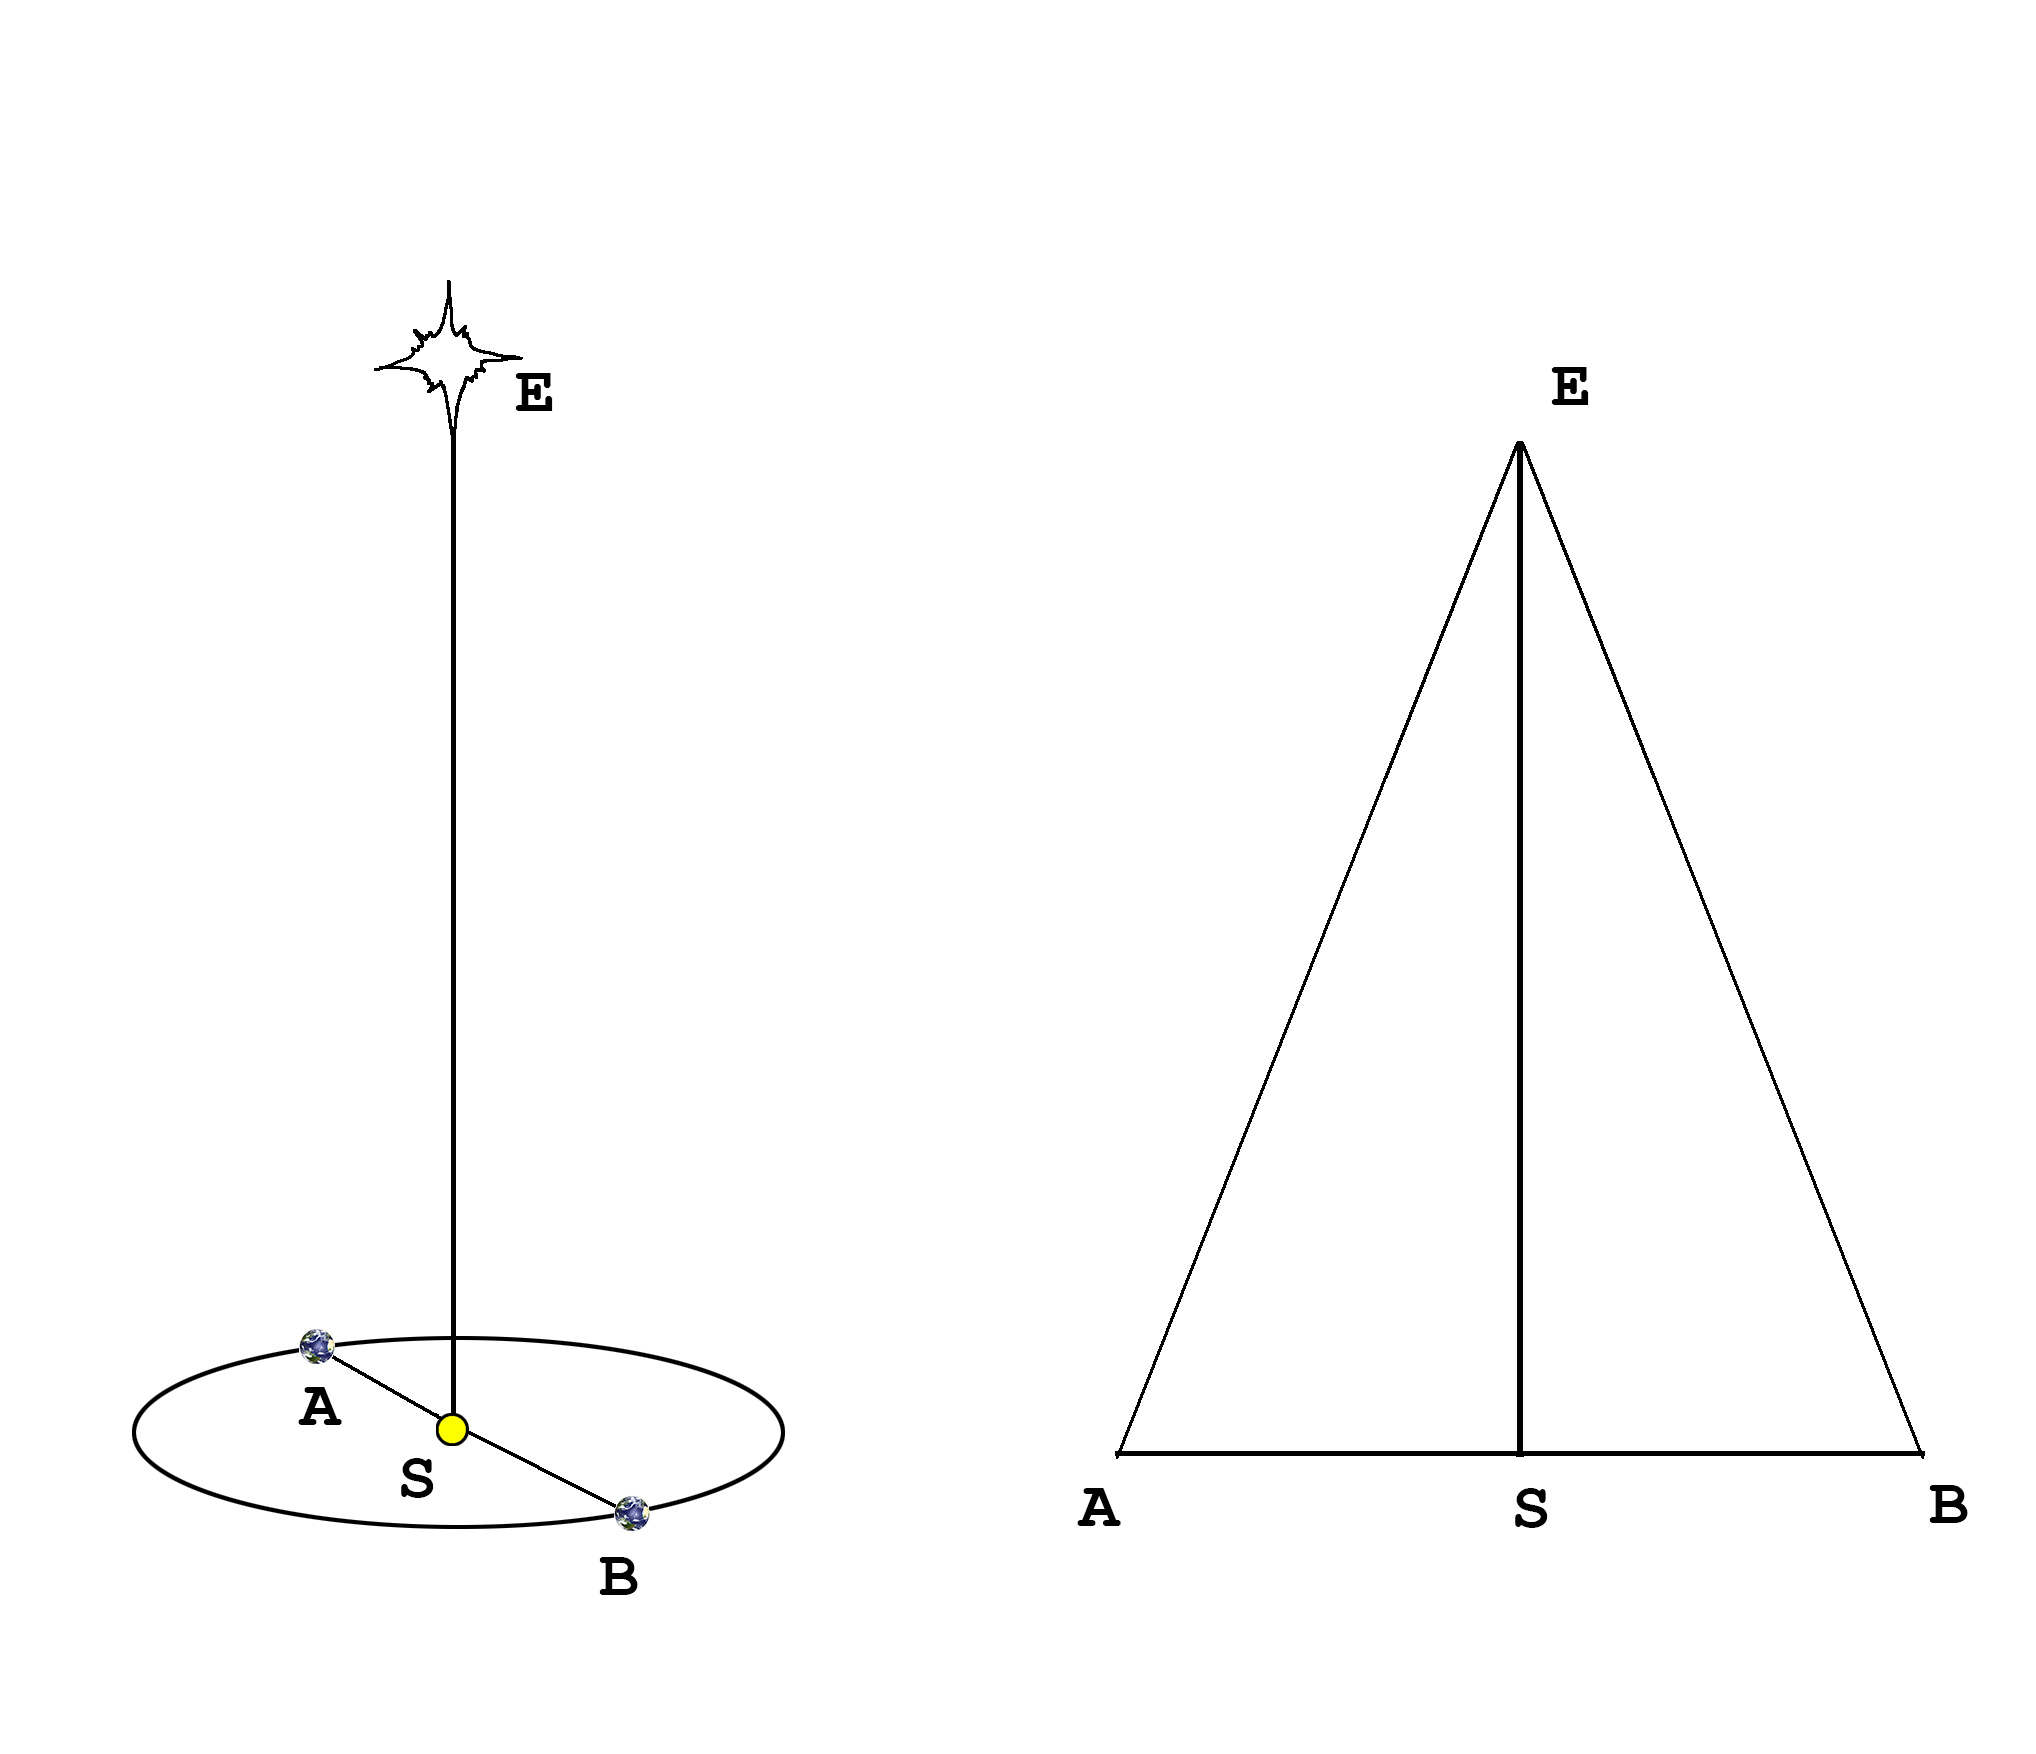
\includegraphics[width=0.6\textwidth]{image/fct_trigo/fig2_parallaxe.jpg}
			\caption{Représentation (pas à l'échelle) d'un cas parcitulier de parallaxe. À gauche\,: figure en perspective. À droite\,: figure plane.}
			\label{fig_par}
		\end{figure}


		Une minute d’arc d’angle mesure un soixantième de degré\,: $1'=\frac{1}{60}^\circ$. Une seconde de degré mesure un soixantième de minute de degré\,: $1''=\frac{1}{60}'$. Ainsi, $1''=\frac{1}{3600}^\circ$. 
		On mesure $\widehat{SEB}=0.02''$. On sait que le rayon de l’orbite terrestre mesure environ $150\cdot 10^6$km.

		\begin{enumerate}
			\item Calculer $EB$ en km.
			\item Si on avait voulu faire un schéma à l’échelle avec $EB=20$cm, combien aurait dû mesurer $AB$ sur le schéma\,? Aurait-on pu faire un schéma à l’échelle sur une feuille A4\,?
			\item Maintenant on s'intéresse à une mesure de parallaxe quelconque (voir figure \ref{fig_par_vrai}). Sachant que l'on mesure les angles $\alpha=\widehat{ST_1E}$, $\beta=\widehat{ST_2E}$, et que l'on connaît le rayon $R$ de l'orbite de la Terre, calculer $T_1E$ et $T_2E$ en fonction des grandeurs connues.
		\end{enumerate}

		\begin{figure}
			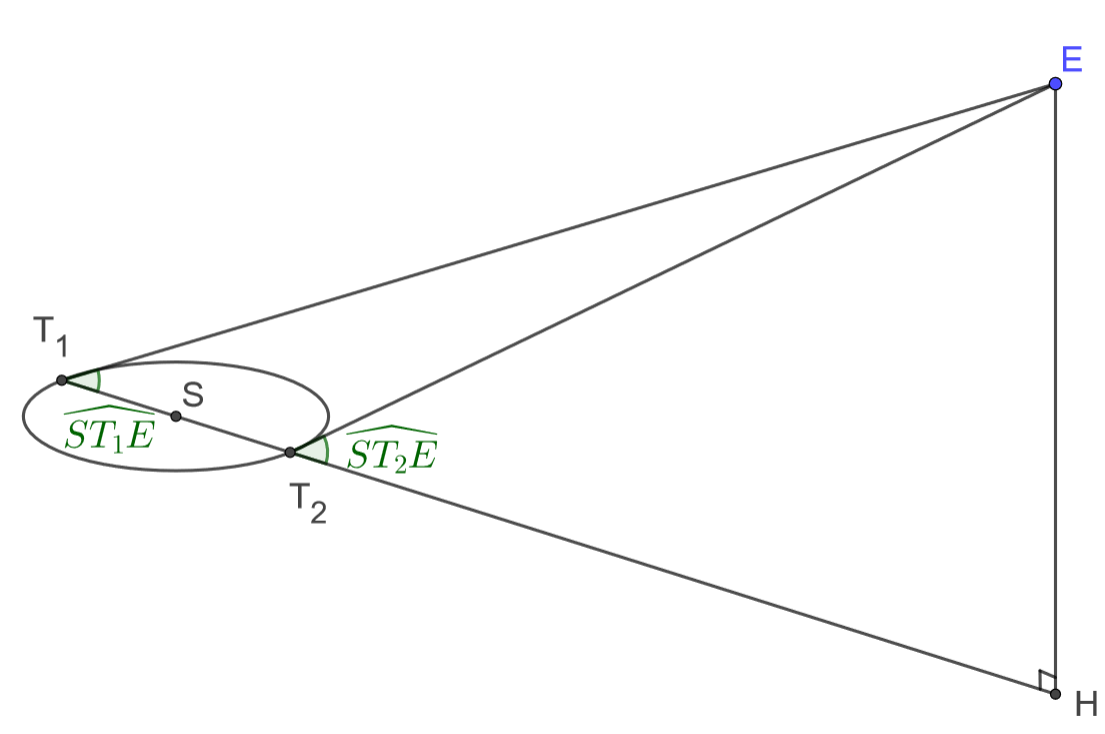
\includegraphics[width=0.6\textwidth]{image/fct_trigo/fig1_parallaxe.png}
			\caption{Situation générale de mesure par parallaxe, en perspective. Les points $T_1$, $S$, $T_2$, $E$, et $H$ sont dans le même plan.}
			\label{fig_par_vrai}
		\end{figure}
